\section{Experiments}
\label{sec:experiments}

\subsection{Hyperparameter Selection}

\begin{figure}[htpb]
  \centering
  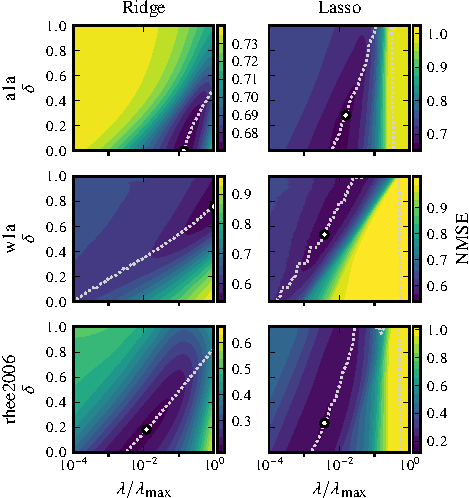
\includegraphics[]{plots/hyperopt_surfaces.pdf}
  \caption{%
    Contour plots of hold-out error across a grid of \(\delta\) and \(\lambda\) values for the
    lasso.
  }
  \label{fig:hyperopt-contours}
\end{figure}

\begin{figure}[htpb]
  \centering
  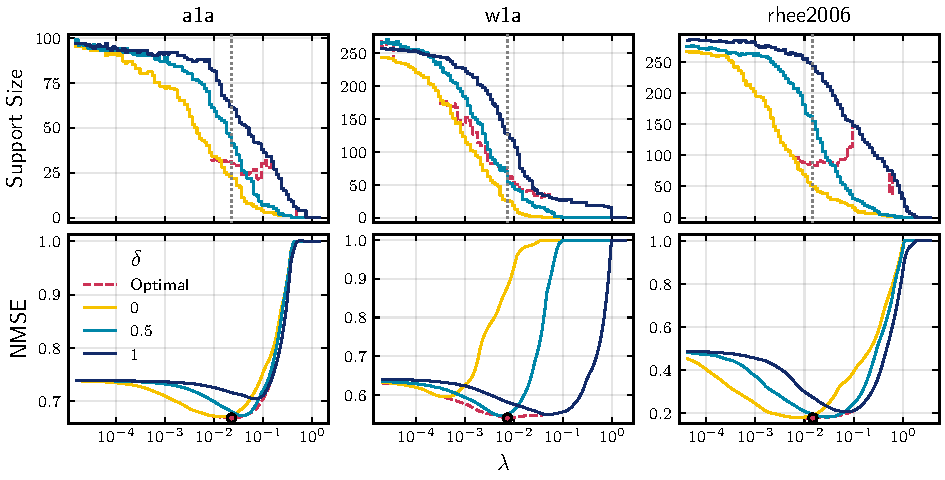
\includegraphics[]{plots/hyperopt_paths.pdf}
  \caption{%
    Support and NMSE of the lasso for different values of \(\delta\) and \(\lambda\).
  }
  \label{fig:hyperopt-support}
\end{figure}

\subsection{Predictive Performance}

\begin{figure}[htpb]
  \centering
  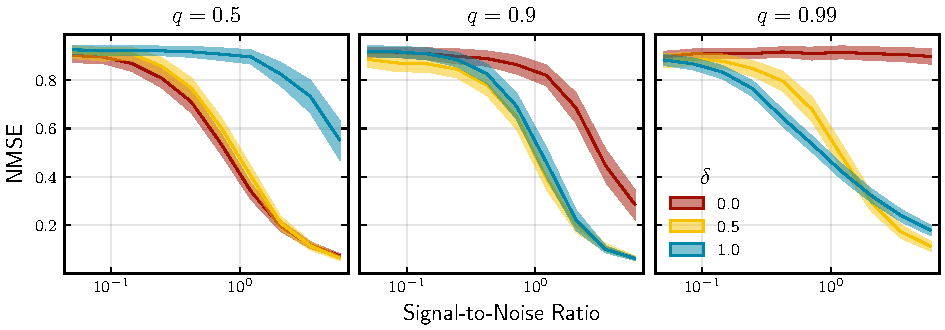
\includegraphics[]{plots/binary_data_sim.pdf}
  \caption{%
    Mean-squared error of \(y - \hat y\) for different types of normalizaion and types of class imbalances in a data set with only binary features.
  }
  \label{fig:binary-sim}
\end{figure}

\begin{figure}[htpb]
  \centering
  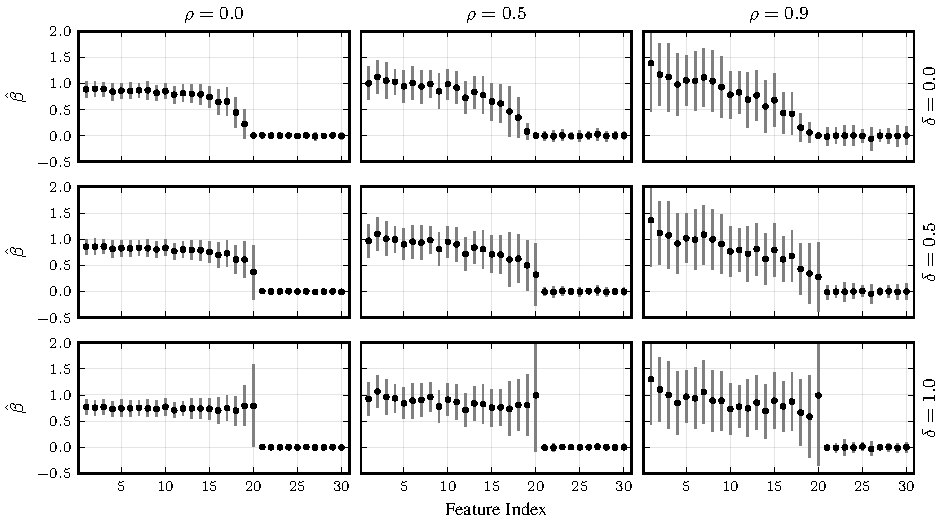
\includegraphics[]{plots/binary_decreasing.pdf}
  \caption{%
    Estimates of the regression coefficients, \(\hat{\vec{\beta}}\), for the first 40 coefficients in the experiment. All of the features are binary and the first 20 features correspond to true signals, with a geometrically decreasing class balance from 0.5 to 0.99. The remaining features have a class balance that's randomly sampled from a uniform distribution with parameters 0.5 and 0.99.}
  \label{fig:binary-decreasing}
\end{figure}

\subsection{Mixed Data}

The next question we now ask ourselves is: given that both features are in the model, what are their respective sizes given differences in class balance (\(q\))?

To begin to answer this question, we conduct simulations on a two-dimensional problem. Along with our previous reasoning, we sample one feature from \(\normal(0, 0.5)\) and the other from \(\bernoulli(q)\), varying \(q\) in \([0.5, 0.99]\) to simulate the effect of class imbalance on the estimates from the model. We compare four different strategies of normalization:
\begin{description}
  \item[Mean-Std] Standardization
  \item[Mean-StdVar] Mean centering and scaling the normal feature by standard deviation and the binary feature by variance
  \item[Mean-Var] Mean centering and scaling each feature by its variance
  \item[None] No normalization
\end{description}

The results~(\Cref{fig:lasso-ridge-comparison}) show that when it comes to ridge, standardization creates class balance-insensitive estimates, whereas for the lasso, this is not the case. For the lasso, it is instead the Mean-StdVar and Mean-Var normalization methods that generate estimates that are insensitive to class imbalances.

\begin{figure}[htpb]
  \centering
  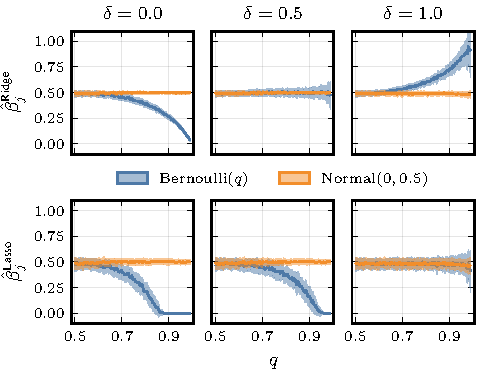
\includegraphics{plots/mixed_data.pdf}
  \caption{%
    Comparison between lasso and ridge estimators for a two-dimensional problem where one feature is generated from \(\bernoulli(q)\) and the other from \(\normal(0, 0.5)\) and the features are normalized in various ways.}
  \label{fig:lasso-ridge-comparison}
\end{figure}

\subsection{Interactions}

\begin{figure}[htpb]
  \centering
  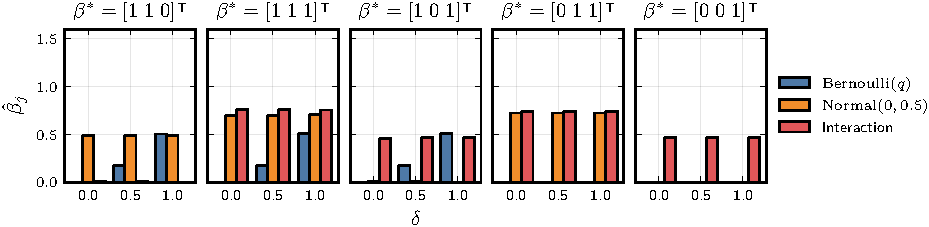
\includegraphics[]{plots/interactions.pdf}
  \caption{%
    The effect of different normalization strategies for mixed data with interactions.
  }
\end{figure}
